\documentclass[11pt]{scrartcl}
\newcommand*\student[1]{\newcommand{\thestudent}{{#1}}}
\newcommand*\course[1]{\newcommand{\thecourse}{{#1}}}
\newcommand*\courseshort[1]{\newcommand{\thecourseshort}{{#1}}}
\newcommand*\assnumber[1]{\newcommand{\theassnumber}{{#1}}}

\student{Stefano Taillefert}
\course{Machine Learning}
\courseshort{ML}
\assnumber{2}

%----------------------------------------------------------------------------------------
%	PACKAGES AND OTHER DOCUMENT CONFIGURATIONS
%----------------------------------------------------------------------------------------

\usepackage[utf8]{inputenc} % Required for inputting international characters
\usepackage[T1]{fontenc} % Use 8-bit encoding
\usepackage[sc]{mathpazo}
\usepackage{caption, subcaption}
\usepackage[hidelinks]{hyperref}
\usepackage{inconsolata}

\usepackage[english]{babel} % English language hyphenation
\usepackage{amssymb}
\usepackage{amsmath}% Math packages
\usepackage{listings} % Code listings, with syntax highlighting
\usepackage{graphicx} % Required for inserting images
\usepackage{float}

%----------------------------------------------------------------------------------------
%	DOCUMENT MARGINS
%----------------------------------------------------------------------------------------

\usepackage{geometry} % For page dimensions and margins
\geometry{
	paper=a4paper, 
	top=2.5cm, % Top margin
	bottom=3cm, % Bottom margin
	left=3cm, % Left margin
	right=3cm, % Right margin
}
\setlength\parindent{0pt}

%----------------------------------------------------------------------------------------
%	SECTION TITLES
%----------------------------------------------------------------------------------------

\usepackage{sectsty}
\sectionfont{\vspace{6pt}\centering\normalfont\scshape}
\subsectionfont{\normalfont\bfseries} % \subsection{} styling
\subsubsectionfont{\normalfont\itshape} % \subsubsection{} styling
\paragraphfont{\normalfont\scshape} % \paragraph{} styling

%----------------------------------------------------------------------------------------
%	HEADERS AND FOOTERS
%----------------------------------------------------------------------------------------

\usepackage{scrlayer-scrpage}
\ofoot*{\pagemark} % Right footer
\ifoot*{\thestudent} % Left footer
\cfoot*{\thecourseshort \ assignment \theassnumber} % Centre footer

%----------------------------------------------------------------------------------------
%	TITLE SECTION
%----------------------------------------------------------------------------------------

\title{	
	\normalfont\normalsize
	\textsc{\thecourse\\%
	Università della Svizzera italiana}\\
	\vspace{25pt}
	\rule{\linewidth}{0.5pt}\\
	\vspace{20pt}
	{\huge Assignment \theassnumber}\\
	\vspace{12pt}
	\rule{\linewidth}{0.5pt}\\
	\vspace{12pt}
}

\author{\LARGE \thestudent}

\date{\normalsize\today}

\begin{document}

\maketitle

%----------------------------------------------------------------------------------------
%%	PROBLEMS - EDIT HERE
%----------------------------------------------------------------------------------------

\section*{Problem 1}

	\begin{figure}[H]
		\centering
		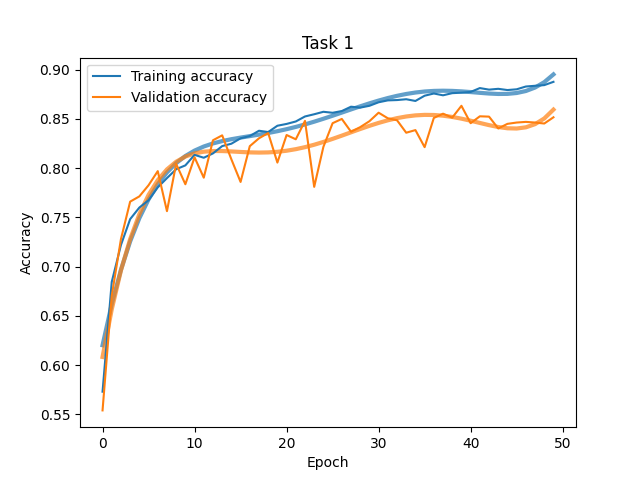
\includegraphics[width=\textwidth]{src/plot_task1.png}
		\caption{The plot for T1}
		\label{fig:plot_T1}
	\end{figure}

	The results from the models are:\\
	
	\begin{table}
		\centering
		\begin{tabular}{cccc}
			Model & Test loss & Accuracy & MSE\\
			\hline
			8 neurons - 0.003 LR & 0.3564 & 0.8576 & 0.0674\\
			16 neurons - 0.01 LR & 0.4255 & 0.8363 & 0.0798\\
			64 neurons - 0.01 LR & 0.4881 & 0.8113 & 0.0920\\
			16 neurons - 0.0001 LR & 0.3692 & 0.8536 & 0.0703\\
			64 neurons - 0.0001 LR & 0.3952 & 0.8416 & 0.0756
		\end{tabular}
	\end{table}

	The best model is the one with 8 neurons - 0.003 LR, the initial one.

	The model is in the file \texttt{deliverable/nn\_task1.h5}, while the code used to 
	generate it is in \texttt{src/create\_models.py}


\section*{Problem 2}

	\subsection*{Without augmentation}

		\begin{figure}[H]
			\centering
			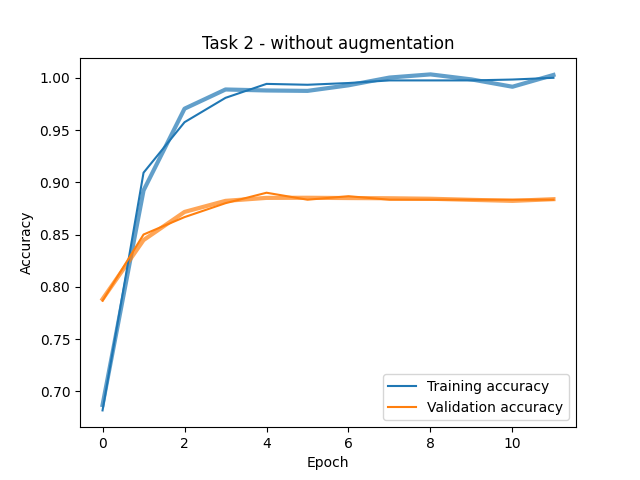
\includegraphics[width=\textwidth]{src/plot_task2_no_augmentation.png}
			\caption{The plot for T2 without augmentation}
			\label{fig:plot_T2_1}
		\end{figure}

		The results from the model without augmentation are:\\
		
		Test loss: 0.2259 - Accuracy: 0.9366 - MSE: 0.0319 (my pc)\\
		Test loss: 0.3201 - Accuracy: 0.9100 - MSE: 0.0464 (colab)\\

		The model is in the files \texttt{deliverable/nn\_task2\_no\_augmentation.h5} and\\ 
		\texttt{deliverable/nn\_task2\_no\_augmentation.pkl}, while the code used to generate 
		it is in \texttt{src/create\_models.py}


	\subsection*{With augmentation}

		\begin{figure}[H]
			\centering
			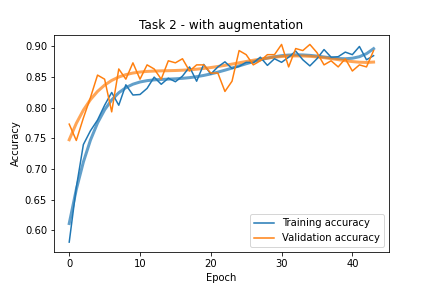
\includegraphics[width=\textwidth]{src/plot_task2_augmentation.png}
			\caption{The plot for T2 with augmentation}
			\label{fig:plot_T2_2}
		\end{figure}

		The results from the model with augmentation are:\\
		
		Test loss: 0.2214 - Accuracy: 0.9133 - MSE: 0.0421 (colab)\\

		The model is in the files \texttt{deliverable/nn\_task2\_augmentation.h5} and\\ 
		\texttt{deliverable/nn\_task2\_augmentation.pkl}, while the code used to generate 
		it is in \texttt{src/create\_models.py}


\section*{Conclusions}

	T1 and first part of T2 ran on my pc, T2 part 2 ran on Colab cause out of VRAM\\

	\texttt{W tensorflow/core/common\_runtime/bfc\_allocator.cc:456] Allocator (GPU\_0\_bfc) ran
	out of memory trying to allocate 3.59GiB (rounded to 3853516800)requested by op
	sequential\_6/vgg16/block1\_conv1/Relu}


\end{document}
